\documentclass[12pt]{article}
\usepackage[utf8]{inputenc}
\usepackage{cite}
\usepackage{listings}
\usepackage[scale=0.75]{geometry}
\usepackage[hidelinks]{hyperref}
\usepackage{graphicx}
\usepackage{xcolor} % for setting colors
\author{Carlos Bergillos, Antoni Rambla, Adrià Cabeza\\ Departament de Computació}
\title{Document similarity detection using hasing }
\date{\today}
\lstset{
    numbers=none,
    commentstyle=\color{red}, % comment color
	breaklines=true,showstringspaces=false,
  	postbreak=\mbox{\textcolor{red}{$\hookrightarrow$}\space},
	tabsize = 2,
	language=C++
}



\begin{document}
  \maketitle  

  \vspace{2cm}
	\begin{abstract}

Our goal is to identify similarities between documents. We have used the Jaccard Similarity theorem,  \textit{Local-Sensitive Hashing} algorithm
 and a \textit{k-shingles} and \textit{minhash signatures} representation of documents to evaluate the effectivity of the similarity computed and the time of computation. We have introduced three different hash functions to see its differences in performance.  Also  once determined the best parameters for the collection, we will give a conclusion about the best way to indentify the more similar documents. 
\end{abstract}

\newpage
\tableofcontents
\newpage

\section{Introduction}

Our goal is to identify similarities between documents. We say that two documents are similar if they contain a significant number of common substrings that are not too small. 

The problem of computing the similarity between two files has been studied extensively and many programs have been developed to solve it. Algorithms for the problem have numerous applications, including spelling correction systems, file comparison tools or even the study of genetic evolution.

 Existing approaces can also include a brute force approach of comparing all sub-strings of pair of documents. However, such and approach is computationally prohibitive. 

 In our case we have represented each document using a k-shingles set of strings, and implemented algorithms to calculate the Jaccard Similarity and an approximation of it using a \textit{Local-Sensitive Hashing} algorithm
 based on \textit{minhash signatures}.


 
\section{Concept of similarity}
First we have to focus into the definition of similarity, when we talk about the ``Jaccard similarity'',which is calculated by looking at the relative size of their intersection. 

The Jaccard similarity, also known as Jaccard index is a statistical measure of similarity of sets. For two sets, it is defined as the size of the intersection divided by the size of the union of the sample sets. Mathematically,
\bigbreak
\centerline{\large $J(A,B)=\frac{\left |A\cap B  \right |}{ \left |A\cup B  \right |} = \frac{\left |A\cap B  \right |}{ \left|A\right|+\left|B\right|-\left |A\cap B  \right |} $}
\bigbreak

Calculating the similarity estimation using this approach could be solved using \textit{k} independent repetitions of the MinHash algorithm, however this would require $O(k \cdot |A|)$ running time. 

The complexity of our implementation is $O(n)$. To calculate the intersection of both sets we two iterators that iterate through both sets. When an element of a set is smaller than the other we increment its iterator and when they are equal we iterate both and a counter. Finally we use the value of the counter to apply the formula. 
\lstset{language= C++}
\begin{lstlisting}
double intersection(const set<string>& A, const set<string>& B){
	int common = 0; 
	auto it = A.begin(), it2 = B.begin();
	while(it!= A.end() and it2 != B.end()){
		if(*it < *it2){
			++it;
		}
		else if(*it > *it2){
			++it2;
		}
		else {
			++it;
			++it2;
			++common;
		}
	}
	return common; 
}

double Jaccard(const set<string>& A, const set<string>& B){
	double size_intersection = intersection(A,B);
	return size_intersection / (A.size() + B.size() - size_intersection);
}

\end{lstlisting}

If we take in account the cost of building a set we should observe that for unsorted sequences our cost would be incremented to $O(n \times log(N))$.


%In the case of finding similarities in text a slightly different approach is required. First, it is important to observe that testing whether two documents are exact duplicates is easy; just comparing the two documents characther-by-character would work. However, even if the documents are not identical, they can share large portions of their text.
\section{Representation of documents}

To identify lexically similar documents we need a proper way to represent documents as sets and the most effective way is to construct from the document the set of short strings that appear within it. If we do so, even if the documents have different sizes or those sentences appear in different order we will find several common elements. In the next section we will introduce some of the approaches of shingling and its variations.

\section{\textit{k}-Shingles}

A k-shingle (or word-k-gram) is a sequence of consecutive words of size k. Intuitively, two documents A and B are similar if they share enough k-shingles. By performing union and intersection operations between the k-shingles, we can find the Jaccard similarity coefficient between A and B. 
\\
There are some variations regarding on how white space (blank, tab, newline, etc) is treated. Also there is a variation that works with a bag of shingles instead of a set to keep the number of appearences of a shingle. \medskip \\
\\
How large k should be depends on how long typical documents are and how large the set of typical characters is. For example if we pick k=4 there are $27^4=531441 $ possible k-shingles. However, the calculation can be a little bit more subtile because all the characters do not appear with equal probability. A good rule of thumb is to imagine that there are only 20 characters and estimate the number of k-shingles as $20^k$. For large documents, choice k = 9 is considered safe. 

\subsubsection{Hashing Shingles}

Instead of using substrings direcly as shingles, we can pick a hash function that maps strings of length k to some number of buckets and treat the resulting bucket number as the shingle. That process compacts our data and lets us manipulate shingles by single-word machine operations.

\section{MinHash}

A minhash function on sets is based on a permutation of the universal set. Given any such permutation, the minhash value for a set is that element of the set that appears first in the permuted order. 

This algorithm provides us with a fast approximation to the Jaccard Similarity. The concept is to condense the large sets of unique shingles into a much smaller representations called ``signatures''. We will then use these signatures to measure the similarity between document, the signature won't give us the exact similarity but we will get a close estimate (the larger the number of signatures you choose, the more accurate the estimate). In this case we define the similarity like: 
\\ \medskip

$$  sim(a,b) = \frac{1}{t} \sum_{i=1}^{t}\left\{
1  \; \; \;  if \; \;  a_{i} = b_{i} \\
\; \; \;  or \; \; \;  0 \; \; \;   if\: \;  a_{i} \neq  b_{i} 
\}\right.  $$


To implement the idea of generating randomly permutated rows, we don’t actually generate the random numbers, since it is not feasible to do so for large datasets, e.g. For a million itemset you will have to generate a million integers …, not to mention you have to do this for each signatures that you wish to generate. One way to avoid having to generate n permutated rows is to pick n hash functions in the form of :
\medbreak
\begin{center}
$ h(x)=(ax+b) mod(c)$
\end{center}

Where: 
\begin{itemize}
\item x is the row numbers of your original characteristic matrix
\item a and b are any random numbers smaller or equivalent to the maximum number of x 
\item c is a prime number slightly larger than the total number of shingle sets. 
\end{itemize}

\section{Locality-Sensitive Hashing for Documents}
 This technique allows us to avoid computing the similarity of every pair of sets or their minhash signatures. If we are given signatures for the sets, we may divide them into bands, and only measure the similarity of a pair of sets if they are identical in at least one band. By choosing the size of bands appropriately, we can eliminate from consideration most of the pairs that do not meet our threshold of similarity.
 \medskip 
 
\subsection{Hash function used to hash a vector}
 \begin{lstlisting}
int hash_vec(V) {
	seed = V.size();
	for each i in V do:
		seed = seed XOR (i + 0x9e3779b9 + (seed << 6) + (seed >> 2));	
		//operands << and >> are shifting left and right respectively x bits
	return seed;
}
\end{lstlisting}
 \medskip 
  
\subsection{Filling the signature matrix}
\begin{lstlisting}
fill(Matrix<unisgned int> repMatrix, set<string> shingles, 
vector<set<string>> docShing){
	set iterator it = shingles.begin();	
	for i = 0 to repMatrix.size() do:
		repMatrix[i][0] = i;
		string shingle = shingles.get(it);
		it++; 
		for j = 1 to repMatrix[0].size() do:
			if(docShing[j-1].contains(shingle))then repMatrix[i][j] = 1;
				//el programa en columna j conte el shingle "shingle"
			else repMatrix[i][j] = 0;
}
\end{lstlisting}
\medskip

\subsection{Get the similarity}
\begin{lstlisting}
float sim(Matrix<unsigned int> signatureMatrix, int a, int b)
    float simil = 0;
    for int i = 0 to signatureMatrix.size() do:
        if(signatureMatrix[i][a] == signatureMatrix[i][b])
						then ++simil;
    
    return simil / signatureMatrix.size();


\end{lstlisting}

\begin{large}Funció que ens ordena un parell posant el més gran com a segon.
\end{large}

\begin{lstlisting}
parella_inc(int a, int b){
	if(a < b ) then return pair(a,b);
	else return pair(b,a);

main()
    set<string> shingles,aux;	
    //set of the total of shingles we have
     and an auxiliar for each document
    vector<set<string>> docShing; 
   //for each document we save its set of shingles
    for i = 1 to number of documents do:
        aux = kshingles(file[i], 9, false, true, true);
        shingles.add(aux);
        docShing[i] = aux;
    Matrix<unsigned int> repMatrix (shingles.size(),
     vector<unsigned int> (numer of files +1 ));
    fill(repMatrix, shingles, docShing);
    int b, r, h;
    cin >> b >> r; //number of bands and rows
    h = r*b;
    Matrix<unsigned int> signatureMatrix
     (h, vector<unsigned int> (number of files, INFINITY));
    hashing of choice
    set<pair<unsigned int,unsigned int>> candidats;                     
    map<unsigned int,vector<unsigned int>> bucket;
    for i = 0 to h do:
        bucket.clear();
        for j = 0 to number of documents do:
            vector<unsigned int> row;
            for k = 0 to r do:
                row.push_back(signatureMatrix[i+k][j]);
                //computing rows
            unsigned int doc1 = hash_vec(row);
			if(bucket.containsKey(doc1)) then
			//we find a row that has the same hash signature
				for l = 0 to bucket[doc1].size() do: 
				//we may have several rows with the same hash signature that 
				//means they are all candidates with each other
					candidats.insert(parella_inc(bucket[doc1][l],j));
				           
            	bucket[doc1].push_back(j);
            else 
            	bucket[doc1] = vector<unsigned int>( 1 , j);
}
 
 \end{lstlisting}
 
\section{Distance Measures}

In this section we shall take a break to study the notions of distance measure.
Suppose we have two points (i.e. x and y), a distance measure on them is a function d(x,y) that produces a real number and satisfies the following properties:
\begin{itemize}
\item d(x,y) $\geq$ 0 

\item d(x,y) = 0 $\iff$ x = y 

\item d(x,y) $\leq$ d(x,z) + d(z,y) (this is called the triangle inequality)
\end{itemize}


\subsection{Jaccard Distance}

We define the Jaccard distance of two sets x and y as d(x,y) = 1 - SIM(x,y). Note that the Jaccard similarity is the probability that a random hash function maps x and y to the \textit{same} value, that means d(x,y) is the probablility that a random hash function sends them to \textit{different} values.

\subsection{Edit Distance}


\section{Hashing}

Hashing is a technique for dimensionality reduction. It uses a hash function that is any function that can be used to map data ( called a key) of arbitrary size to data of a fixed size (called a hash value or hash). That hash is a sum up of everything that is in the data. You can never make it backwards from the hash to the data.

Hashing is done for indexing and locating items in databases because it is easier to find the shorter hash value than the longer string.

The hash functions that we want to use need to be: 

\begin{itemize}
\item \textbf{Really fast}\\
Dimensionality reduction is often a time bottle-neck and using a fast basic hash function to implement it may improve running times significantly. 
\item \textbf{Avoid hash collisions}\\
We do not want to get the same hash using different pieces of data %(DIR ALGU DEL pidgeon hole principle)
\item \textbf{Uniform distribution}\\
The hash values are uniformly distributed.
%TODO: mirar, no estic segur de quines característiques necessitem, també he vist altres distribucions, en llop va ficar també que fossin independents

\end{itemize}

In our project we have not choosen hash cryptographic functions (i.e. sha-1 or md5) because they are too slow for our purpose.

\subsection{Modular Hashing}

In the modular hashing (also called the division method), we map a key $k$ into one of $m$ slots by taking the reminder of k divided by m. It takes the following form. 

\begin{center} $h(k) = k (mod (m))$ \end{center}

When using the division method, we usually avoid certaing values of $m$. For example, $m = 2^p$ for some integer $p$, then $h(k)$ would be just the $p$-lowest-order bits of $k$. A prime value is often a good choice of $m$.



\subsection{Multiplicative Hashing}
The multiplicative method for creating hash functions operates in two steps.
Firstly, we multiply the key $k$ by a constant $A$ in the range $0<A<1$ and extract the fractional part of $kA$. Then, we multiply this value by $m$ and take the floor the result. To sum up:  

\begin{center}
 $ \lfloor m\ kA \times mod(1)  \rfloor$
\end{center}
Where:
\begin{itemize}
\item $kA  \times mod(1)$  is the fractional part of $kA$, that is, $kA- \lfloor kA \rfloor$
\end{itemize}
An advantage of the multiplication method is that the value of m is not critical. We typically choose it to be a power of 2 ($m = 2^p$ for some integer $p$), since we can then easily implement the function on most computers.
\\

\begin{center}
\begin{large}
Pseudocode 
\end{large}
\end{center}

\begin{lstlisting}[mathescape=true]
MultiplicativeHashing(k,len)

	$A \leftarrow (\sqrt{5} -1)/2 \simeq 0.6180339887 $
	$s \leftarrow A\times 2^w$
	$r \leftarrow k \times s$ 
	$r_0 \leftarrow r\ mod\  (2^w) $ 
	$value \leftarrow r_0 >> (w-len)$

\end{lstlisting}

\vspace{0.7cm}
Supposing that the word size of the machine is $w$ bits, that $k$ fits in a single word and $len$ is the number of bits that you want for the size of your hash value.

 We restrict $A$ to be a fraction of the form, where s is an integer in the range $0<s<2^w$. We first mulitply k by the w-bit integer $s = A\times 2^w$. The result is a $|2 \times w| $-bit value. The desired len-bit hash value consists of the len most significant bits of $r_0$. 

%\includegraphics[scale=1]{multiplicative.pdf} 

Although this method works with any value of the constant A, it works better with some values than with others. The optimal choice depends on the characteristics of the data being hashed. Donald Knuth suggest that...

$ A = (\sqrt{5} -1)/2 \simeq 0.6180339887  $

...is likely to work well. So that's why we used this value as an starting point to generate different multiplicative hash functions.


\subsubsection{Murmur Hash}

Consists in applying some multiplications (MU) and rotations (R) to the entry bytes to obtaint the hash. It uses multiple constants which are decided to make it a good hash function by passing 2 basic tests, the Avalanche Test that evaluates how the output changes if the input is slightly modified and the statistical Chi-Squared Test. We have based the implementation of this hash function on Austin Appleby's implementation. Souce : \url{https://sites.google.com/site/murmurhash/}\\
\medskip
\begin{center}
\begin{large}
Pseudocode extracted from Wikipedia
\end{large}
\end{center}

\begin{lstlisting}[mathescape=true]
Murmur3(key, len, seed)
    c1 $\leftarrow$ 0xcc9e2d51
    c2 $\leftarrow$ 0x1b873593
    r1 $\leftarrow$ 15
    r2 $\leftarrow$ 13
    m $\leftarrow$ 5
    n $\leftarrow$ 0xe6546b64
 
    hash $\leftarrow$ seed

    for each fourByteChunk of key
        k $\leftarrow$ fourByteChunk

        k $\leftarrow$ k $\times$ c1
        k $\leftarrow$ (k ROL r1)
        k $\leftarrow$ k $\times$ c2

        hash $\leftarrow$ hash XOR k
        hash $\leftarrow$ (hash ROL r2)
        hash $\leftarrow$ hash $\times$ m + n

    with any remainingBytesInKey
        remainingBytes $\leftarrow$ remainingBytes $\times$ c1
        remainingBytes $\leftarrow$ (remainingBytes ROL r1)
        remainingBytes $\leftarrow$ remainingBytes $\times$ c2

        hash $\leftarrow$ hash XOR remainingBytes
 
    hash $\leftarrow$ hash XOR len
    hash $\leftarrow$ hash XOR (hash >> 16)
    hash $\leftarrow$ hash $\times$ 0x85ebca6b
    hash $\leftarrow$ hash XOR (hash >> 13)
    hash $\leftarrow$ hash $\times$ 0xc2b2ae35
    hash $\leftarrow$ hash XOR (hash >> 16)

\end{lstlisting}

\section{Data} %canviar el nom de la secció

\subsection{Real-world data}
\begin{itemize}
\item \textbf{Harry Potter and the Sourcerer Stone}: All the text from the first Harry Potter novel.
\item \textbf{The Lord of The Rings: The return of the King}: The entire script from the last Lord of the Rings movie.
\item \textbf{Star Wars: Heir to the Empire}:  An Star Wars novel by Timothy Zahn. 
\end{itemize}

\subsection{Generating the data}

To generate the data for our experiments we have used the random\_shuffle function inside the C++ STL which rearranges the elements randomly. The function swaps the value of each element with that of some other randomly picked element. Its complexity is $O(n)$ with $n$ being  the distance between first and last minus one.

\begin{lstlisting}

ifstream inFile;
ofstream outFile;

void writeVector(const vector<string>& A, int i,string nameFile){
    outFile.open(nameFile);
    for(int j = 0; j < A.size(); ++j){
        outFile << A[j]<< space symbol;
    }
    outFile.close();
}

int main(){
    int n; 
    cin>>n; //number of permutations that we want to create
         
    string nameFile;
    cin>> nameFile; 
    inFile.open(nameFile); //open the file
    
    vector<string> words; 
    string testline;
    while( inFile >> testline){
    	words.push_back(testline); 
    	//insert each word in a vector of strings
    }
    inFile.close();
    for(int i = 0; i<n;++i){
    	random_shuffle(words.begin(),words.end()); 
    	writeVector(words,i,nom);
    }
    
}\end{lstlisting}


As it can be seen, we traverse all the document once to generate a vector of strings containing all the words and then we shuffle the vector and write the result in a document n times. \\

\section{Experiments}

Vamos a poner unos cuantos experimentos

%\begin{figure}[h]
%	\includegraphics[scale=1]{JaccardSimilarityValueKshingles} 
%  \caption{Relation between the k-shingles and the similarity outputed}
%  \label{fig:KShinglesSimilarity}
%\end{figure}
%
%\begin{figure}[h]
%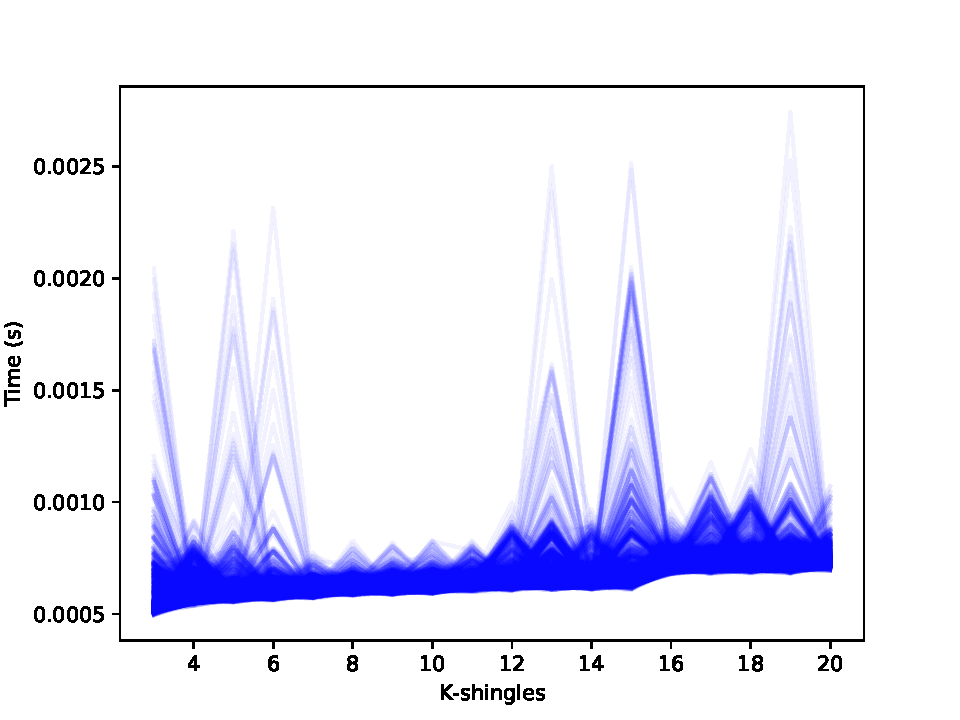
\includegraphics[scale=1]{JaccardSimilarityTimeKshingles.pdf}
%  \caption{Relation between the k-shingles and the time of execution}
%  \label{fig:KShinglesTime}
%\end{figure}



\section{Conclusion}

%http://ethen8181.github.io/machine-learning/clustering_old/text_similarity/text_similarity.html

%mirar aquest algoritme: http://www.xmailserver.org/diff2.pdf
\newpage

\begin{thebibliography}{100}

\bibitem{Concept of similarity}
J.\ Bank and B.\ Cole,
\textit {Calculating the Jaccard similarity coefficient with map reduce for entity pairs in
Wikipedia} (Wikipedia Similarity Team, 2008).

\bibitem{Cambridge}
J.\ Leskovec, A.\ Rajaraman and J.\ Ullman
\textit{ Finding Similar Items. In Mining of Massive Datasets} (Cambridge University Press, 2014).

\bibitem{O(ND) Difference Algorithm}
E.\ W. Myers \textit{An O(ND) Difference Algorithm and Its Variations} (Department of Computer Science, University of Arizona)

\bibitem{Plagiarism Detection}
S.\ Alzahrani and N. \ Salim, \textit{Fuzzy Semantic-Based String Similarity for Extrinsic Plagiarism Detection} (Taif University, Saudi Arabia and Universiti Teknologi Malaysia, Malaysia)

\bibitem{Hash Functions}
S.\ Dahlgaard, M.\ Tejs Knudsen and M.\ Thorup, \textit{Practical Hash Functions for Similarity Estimation and Dimensionality Reduction} (University of Copenhagen)

\bibitem{Universal string hashing}
D.\ Lemire and O.\ Kaser, \textit{Strongly universal string hashing is fast} (Université du Québec Canadá and University of New Brunswick, Canada) 

\bibitem{C++ STL}
C++ Standard Template Library,
\ Source: \url{cplusplus.com/reference/stl/}


\bibitem{MurmurHash, Wikipedia}
\textit{MurmurHash} \ Source: \url{https://en.wikipedia.org/wiki/MurmurHash}

\bibitem{Introduction to Algorithms}
T.\ H.\ Cormen, C.\ E.\ Leierson, R.\ L.\ Rivest and C.\ Stein, \textit{Introduction to Algorithms. Third Edition}

\bibitem{Sorting and searching}
D.\ Knuth,
\textit {Sorting and Searching}, volume 3 of \textit{The Art of Computer Programming} (Addison-Wesley, 1997. Third Edition)


\bibitem{Murmur Hash explained}
S.\ Yar [Developer's Catalog By Sahib Yar]
\textit {Sorting and Searching}, \textit{Murmur Hash - Explained} (Youtube, Jun 23, 2017), Retrieved from: \url{https://www.youtube.com/watch?v=b8HzEZt0RCQ&t=1s}

\bibitem{Hashing Algorithms}
T.\ Scoot [Computerphile]
\textit {Hashing Algorithms and Security - Computerphile}, (Youtube, Nov 8, 2013), Retrieved from: \url{https://www.youtube.com/watch?v=b4b8ktEV4Bg&t=181s}



\end{thebibliography}

\end{document}



\end{thebibliography}

\end{document}

